\chapter{Results and Discussion}\label{ch5:chapter5}


\section{Experiments results Database }\label{ch5:database}

The main objective of this study was to propose an evaluation of three failure criteria for a selected rock, Dunnville Sandstone. As explained in the previous chapters, their empirical nature requires a thick database of diverse multi axial experiments for their development. 

Dunnville Sandstone have been used for several works in the past and particularly for multi axial experiments \cite{Labuz2018}\cite{Zeng2019}\cite{Tarokh2016}. The ones performed in the scope of this study (cf. Chapter \ref{ch4:title}) presented the opportunity to enrich the existing tests results database and to evaluate the failure criteria with data representative of Dunnville Sandstone response.

The database presented in Table \ref{tb5:database} was based on the one proposed by Zeng et al. (2019) \cite{Zeng2019}, and extended with the results of the experiments from this study. In this table, each experiment is associated with the following elements: the orientation of the bedding regarding the application of the axial stress, the three principal stresses (i.e. $\sigma_I$,$\sigma_{II}$,$\sigma_{III}$) and the stress invariants (i.e.$p$, $q$, $\theta$).

This database was used for the evaluation of Mohr-Coulomb,Hoek-Brown and Paul-Mohr-Coulomb failure criteria, that will be presented in the following sections.

\begin{table}
    \centering
    \begin{tabular}{cccccccc}
        \hline 
        Test & Bedding & $\sigma_I$ [\si{MPA}] & $\sigma_{II}$ [\si{MPA}] &$\sigma_{III}$ [\si{MPA}] & $p$ [\si{MPA}] & $q$ [\si{MPA}] & $\theta$ [\si{\degree}] \\
        \hline
        \hline
        Published TC-1 & \(\perp\) & 29.7 & 0.0 & 0.0 & 9.9 & 29.7 & 0 \\
        Published TC-2 & \(\perp\) & 39.4 & 2.5 & 2.5 & 14.8 & 36.9 & 0 \\
        Published TC-3 & \(\perp\) & 52.9 & 5.0 & 5.0 & 21.0 & 47.9 & 0 \\
        Published TC-4 & \(\perp\) & 71.5 & 10.0 & 10.0 & 30.5 & 61.5 & 0 \\
        Published TC-5 & \(\perp\) & 98.4 & 20.0 & 20.0 & 46.1 & 78.4 & 0 \\
        Published TC-6 & \(\perp\) & 114.5 & 30.0 & 30.0 & 58.2 & 84.5 & 0 \\
        Published TC-7 & \(\perp\)& 129.4 & 40.0 & 40.0 & 69.8 & 89.4 & 0 \\
        Published TC-8 & \(\perp\) & 142.1 & 50.0 & 50.0 & 80.7 & 92.1 & 0 \\
        Published TC-9 & \(\perp\) & 153.8 & 60.0 & 60.0 & 91.3 & 93.8 & 0 \\
        Published TC-10 & \(\|\) & 24.9 & 0.0 & 0.0 & 8.3 & 24.9 & 0 \\
        Published TC-11 & \(\|\) & 35.2 & 2.5 & 2.5 & 13.4 & 32.7 & 0 \\
        Published TC-12 & \(\|\) & 48.8 & 5.0 & 5.0 & 19.6 & 43.8 & 0 \\
        Published TC-13 & \(\|\) & 68.0 & 10.0 & 10.0 & 29.3 & 58.0 & 0 \\
        Published TC-14 & \(\|\) & 95.9 & 20.0 & 20.0 & 45.3 & 75.9 & 0 \\
        Published TC-15 & \(\|\) & 110.9 & 30.0 & 30.0 & 57.0 & 80.9 & 0 \\
        Published TC-16 & \(\|\) & 125.5 & 40.0 & 40.0 & 68.5 & 85.5 & 0 \\
        Published TC-17 & \(\|\) & 138.1 & 50.0 & 50.0 & 79.4 & 88.1 & 0 \\
        Published TC-18 & \(\|\) & 150.8 & 60.0 & 60.0 & 90.3 & 90.8 & 0 \\
        UCS   & \(\perp\) & 29.8 & 0 & 0   & 27.95 & 51.43 & 0 \\ 
        TC 9  & \(\perp\) & 49.43 & 5  & 5 & 19.81 & 44.43 & 0 \\ 
        TC 0  & \(\perp\) & 61.43 & 10 & 10 & 27.95 & 51.43 & 0 \\ 
        TC 5  & \(\perp\) & 91.08 & 20 & 20 & 44.72 & 71.08 & 0 \\ 
        TC 8  & \(\perp\) & 127.3 & 40 & 40 & 65.73 & 87.30 & 0 \\ 
        TC 10 & \(\perp\) & 151.1 & 60 & 60 & 88.12 & 91.10 & 0 \\ 
        \hline
        \hline
        Published TE-1 & \(\perp\) & 35.0 & 35.0 & 0.8 & 23.6 & 34.2 & 60 \\
        Published TE-2 & \(\perp\) & 40.0 & 40.0 & 1.2 & 27.1 & 38.8 & 60 \\
        Published TE-3 & \(\perp\) & 50.0 & 50.0 & 6.0 & 35.3 & 44.0 & 60 \\
        Published TE-4 & \(\perp\) & 60.0 & 60.0 & 10.1 & 43.4 & 49.9 & 60 \\
        Published TE-5 & \(\perp\) & 69.0 & 69.0 & 11.5 & 49.8 & 57.5 & 60 \\
        Published TE-6 & \(\|\) & 40.0 & 40.0 & 1.8 & 27.3 & 38.2 & 60 \\
        Published TE-7 & \(\|\) & 50.0 & 50.0 & 5.7 & 35.2 & 44.3 & 60 \\
        Published TE-8 & \(\|\) & 60.0 & 60.0 & 8.0 & 42.7 & 52.0 & 60 \\
        TE 3  & \(\perp\) & 35 & 35 & 3.96 & 24.64 & 31.08 & 60 \\ 
        TE 1  & \(\perp\) & 40 & 40 & 4.50 & 27.89 & 36.34 & 60 \\ 
        TE 2  & \(\perp\) & 60 & 60 & 9.68 & 43.01 & 50.98 & 60 \\
        \hline
        \hline
        Published TT-1 & \(\perp\) & 48.3 & 31.6 & 5.0 & 28.3 & 37.8 & 37.5 \\
        Published TT-2 & \(\perp\) & 52.9 & 25.1 & 7.0 & 28.3 & 40.1 & 22.7 \\
        Published TT-3 & \(\perp\) & 63.9 & 12.1 & 9.0 & 28.3 & 53.4 & 2.9 \\
        Published TT-4 & \(\perp\) & 70.6 & 49.4 & 15.0 & 45.0 & 48.7 & 37.8 \\
        Published TT-5 & \(\perp\) & 77.5 & 70.5 & 20.0 & 56.0 & 54.3 & 53.5 \\
        Published TT-6 & \(\perp\) & 83.9 & 62.1 & 22.0 & 56.0 & 54.4 & 39.7 \\
        TT 1 & \(\perp\) & 88.14 & 46.85 & 10 & 48.33 & 55.28 & 28.12 \\
        TT 2 & \(\perp\) & 99.98 & 20 & 20 & 46.65 & 62.28 & 0 \\
        \hline
    \end{tabular}
    \caption{Database of experiments results for Dunnville Sandstone. The "Published" data are from Zeng et al. \cite{Zeng2019}}
    \label{tb5:database}
\end{table}

%%%%%%%%%%%%%%%%%%%%%%%%%%%%%%%%%%%%%%%%%%%%%%%%%%%%%%%%%%%%%%
\section{Evaluation of the failure criteria}\label{ch5:evaluation}

The Mohr-Coulomb, Hoek-Brown and Paul-Mohr-Coulomb failure criteria presented in Chapter \ref{ch2:title} were fitted to the experiment results of Dunnville Sandstone from Table \ref{tb5:database}. A computation program was developed for the fittings using the programming language Python. All the resources needed to access the program files are listed in Appendix REF{APPENDIX B}. 

The three failure criterion fittings are evaluated through their representation in the three coordinates systems presented in Chapter \ref{ch2:title}, and their accuracy in terms of how good they fit the data. In this study, this "accuracy" is chosen to be evaluated by comparing the least mean standard deviation misfits, as proposed by Benz et al. (2008) \cite{Benz2008}. 

The standard deviation $s_{i}$ of one test series $i$ formed by $j$ experiments subject to the same minor stress (i.e. $\sigma_{III}$) is defined by Equation \ref{eq5:standdev}. In this expression, $n$ is the number of experiments in the test series $i$, $\sigma_{I,j}^{\mathrm{test}}$ is the maximum stress at failure for a data point $j$ (obtained from the database) and $\sigma_{I,j}^{\mathrm{calc}}$ is the calculated one using the considered criterion formulation. 

\begin{equation}\label{eq5:standdev}
    s_{i}=\sqrt{\frac{1}{n} \sum_{j}\left(\sigma_{I,j}^{\mathrm{calc}}-\sigma_{I,j}^{\mathrm{test}}\right)^{2}}
\end{equation}

Finally, the mean standard deviation misfit is computed following Equation \ref{eq5:mean_standdev}, where $m$ is the number of test series. The smallest the $\bar{S}$ is , the better is the "accuracy" of the model for the rock compared to other criteria. 

\begin{equation}\label{eq5:mean_standdev}
    \bar{S}=\frac{1}{m} \sum_{i} s_{i}
\end{equation}


%%%%%%%%%%%%%%%%%%%%%%%%%%%%%%%%%%%%%%%%%%%%%%%%%%%%%%%%%%%%%%
\subsection{Mohr-Coulomb failure criterion}

The Mohr-Coulomb failure criterion is formulated in terms two principal stresses (cf. Equations \ref{eq2:MCfinalform} and \ref{eq2:MCcondenseform}) and unique strength parameters (i.e. $\phi$,$c$), therefore, the fitting was done using only axisymmetric triaxial compression tests results (i.e. $\theta = 0^\circ$). 

From this fitting, the coefficient $K_p$ was determined and the other parameters were computed: 
\begin{equation}
    K_p = 2.55 \quad \textrm{and} \quad C_0 = \SI{29.7}{\mega\pascal}
\end{equation}
\begin{equation}
    \phi = \frac{K_p-1}{K_p+1} = 25.9^\circ
\end{equation}
\begin{equation}
    c = \frac{C_0(1-sin\phi)}{2cos\phi} = \SI{9.30}{\mega\pascal}
\end{equation}
\begin{equation}
    V_0 = \frac{C_0}{K_p-1} = \SI{19.2}{\mega\pascal}
\end{equation}

Knowing the strength parameters, the Mohr-Coulomb failure surface is plotted in the $(\sigma_3-\sigma_1)$ plane using Equation \ref{eq2:MCfinalform}(cf. Figure \ref{fig5:mc_sig1sig3}).

\begin{figure}[tb]
    \centering
    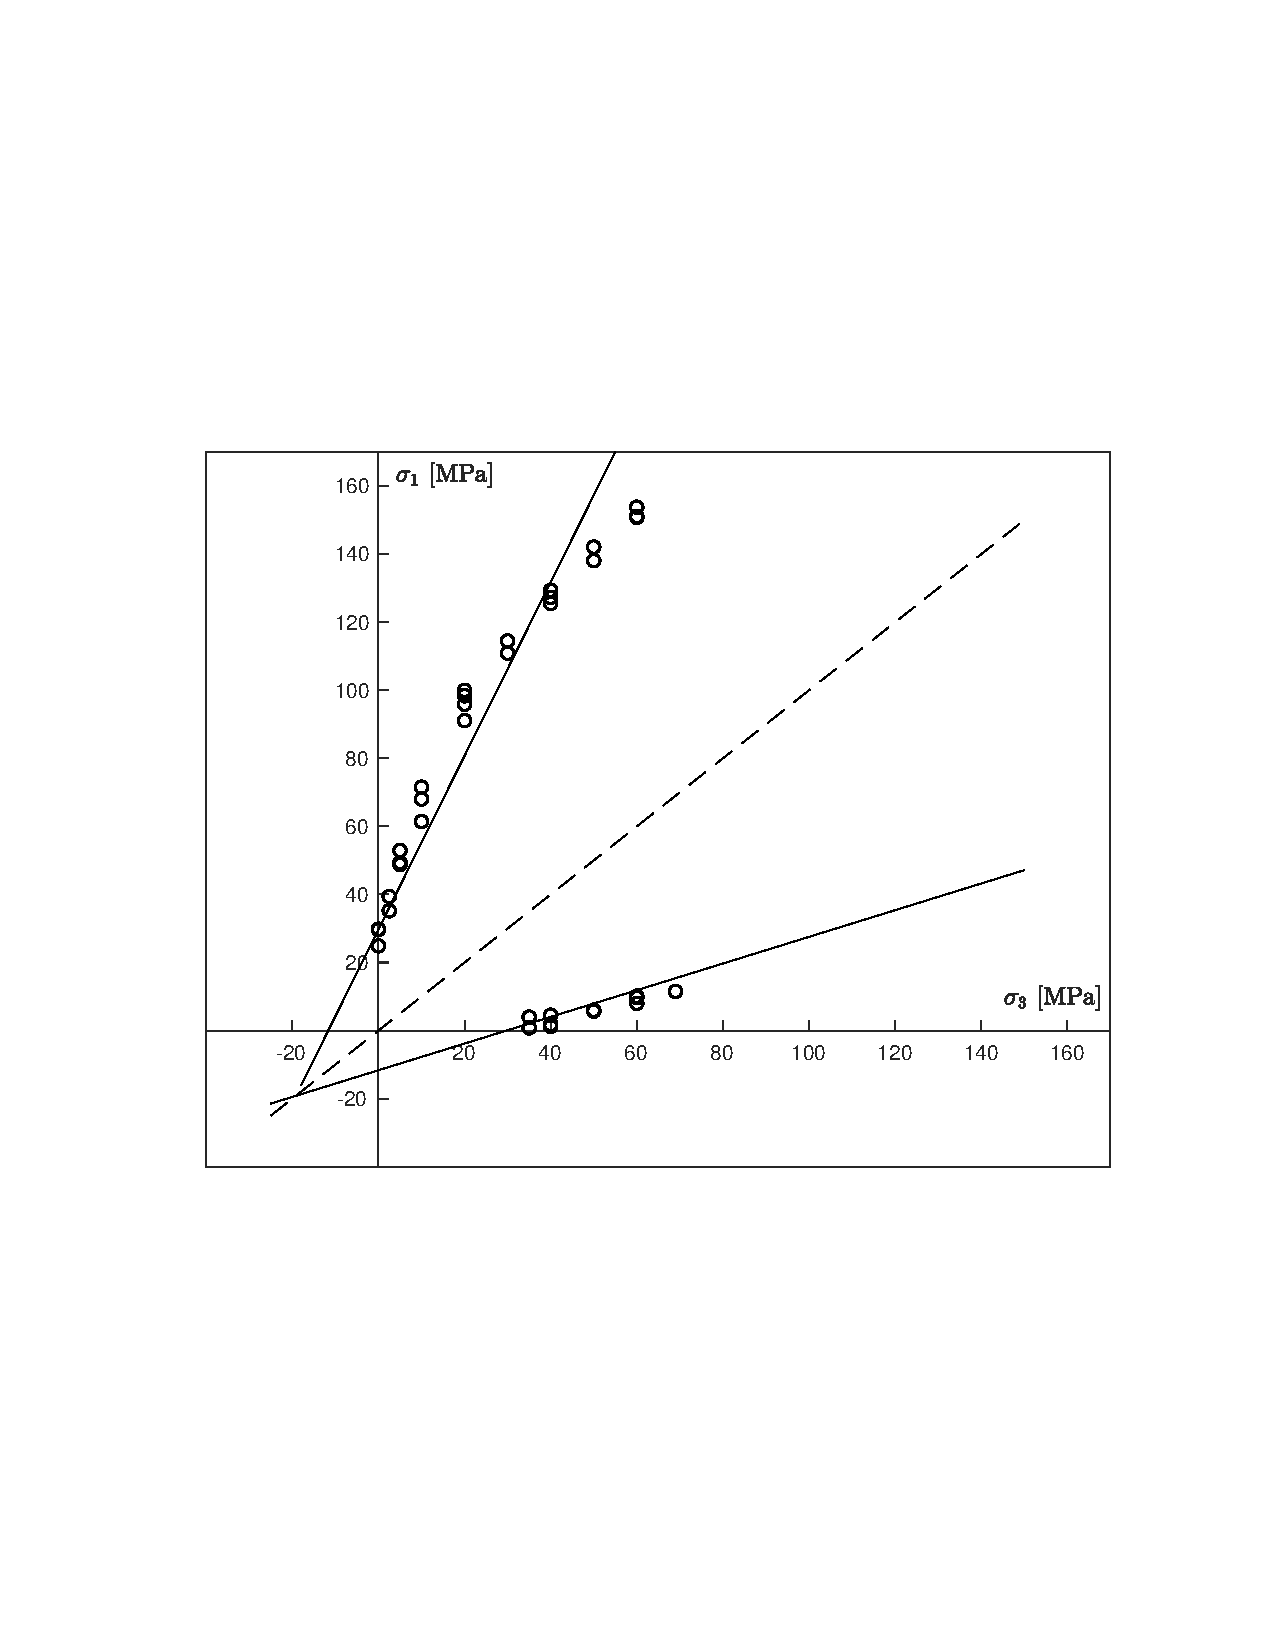
\includegraphics[width=0.8\columnwidth]{ch5/mc_sig1sig3}
    \caption{Mohr-Coulomb criterion failure surface in  $(\sigma_3-\sigma_1)$ plane}
    \label{fig5:mc_sig1sig3}
\end{figure} 

The criterion was also fitted in the $(p-q)$ plane, for which the plot obtained is shown in Figure \ref{fig5:mc_pq}. The coefficients $m_{c,e}$ and $b_{c,e}$ were computed using Equations \ref{eq2:MC_mc_q} to \ref{eq2:MC_be_q}:

\begin{equation}
    m_c = \frac{6 \sin \phi}{3-\sin \phi} = 1.02
\end{equation}
\begin{equation}
    m_e = \frac{6 \sin \phi}{3+\sin \phi} = 0.76
\end{equation}
\begin{equation}
    b_c = \frac{6 c \cos \phi}{3-\sin \phi} = \SI{19.6}{\mega\pascal}
\end{equation}
\begin{equation}
    b_e = \frac{6 c \cos \phi}{3+\sin \phi} = \SI{14.6}{\mega\pascal}
\end{equation}

\begin{figure}[tb]
    \centering
    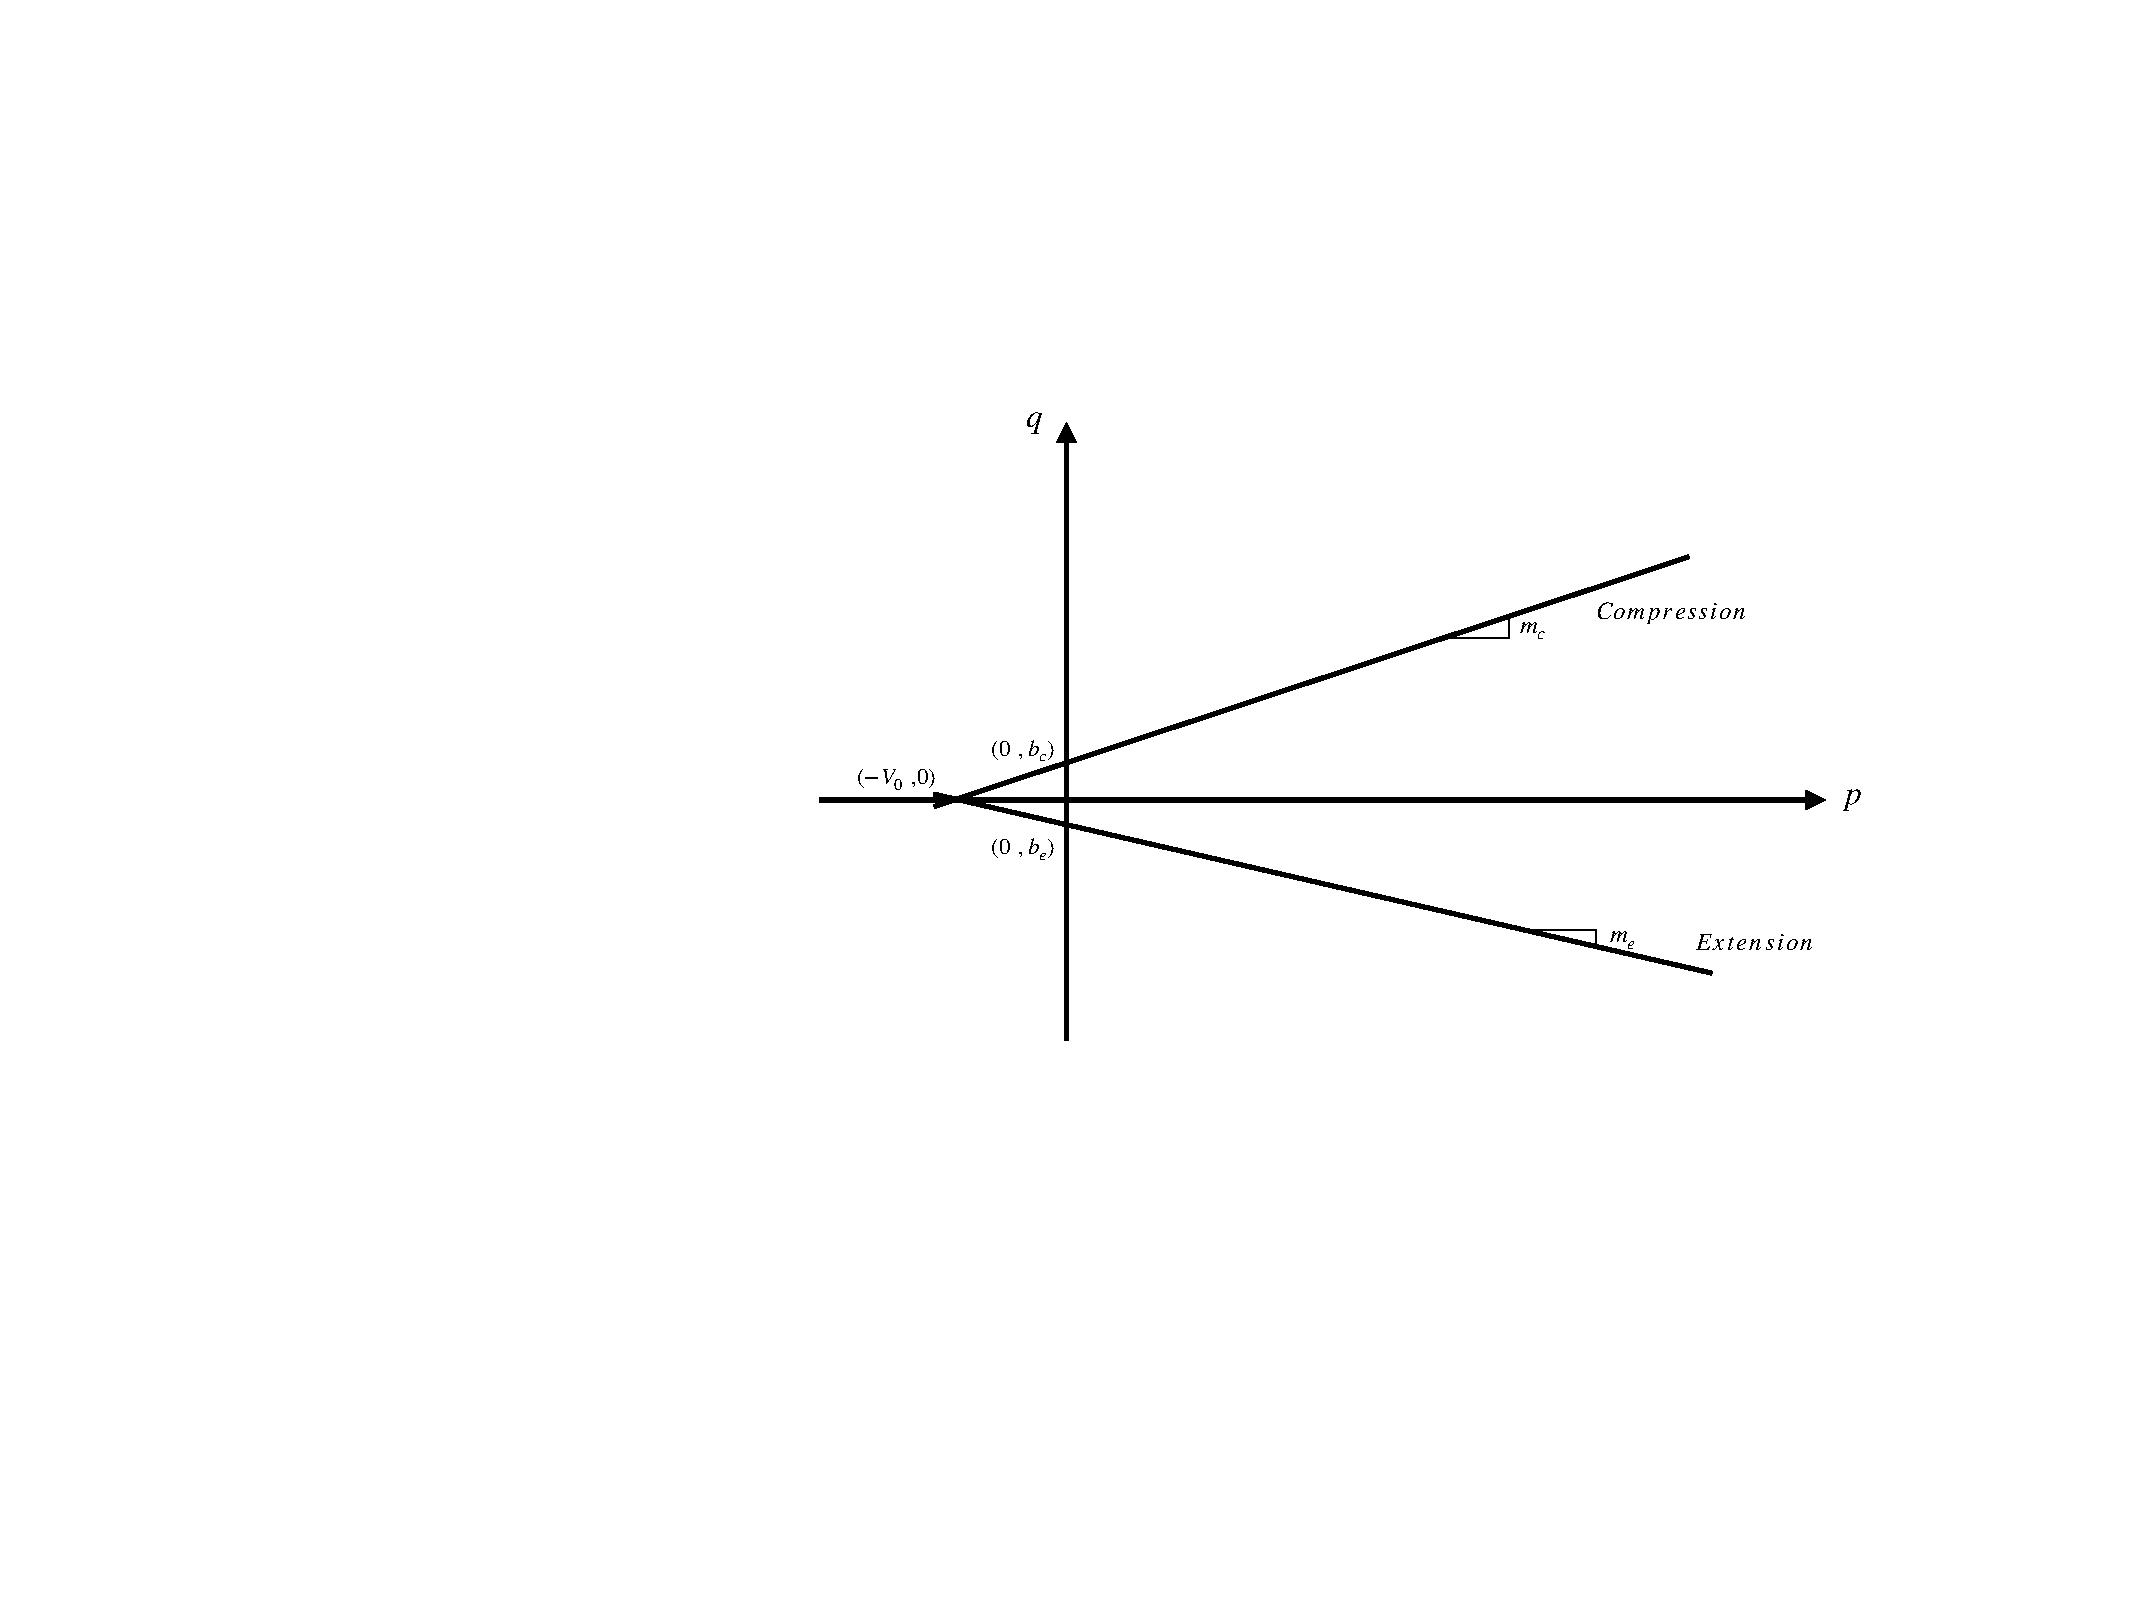
\includegraphics[width=0.8\columnwidth]{ch5/mc_pq}
    \caption{Mohr-Coulomb criterion failure surface in  $(p-q)$ plane}
    \label{fig5:mc_pq}
\end{figure} 

Finally, the Mohr-Coulomb criterion is presented in the $\pi$-plane, obtained following the procedure described in Section \ref{ch2:MC_pi}. Figure \ref{fig5:mc_pi_plane} shows Mohr-Coulomb failure criterion in the pi-plane at different values of the mean stress $p$.

\begin{figure}[tb]
    \centering
    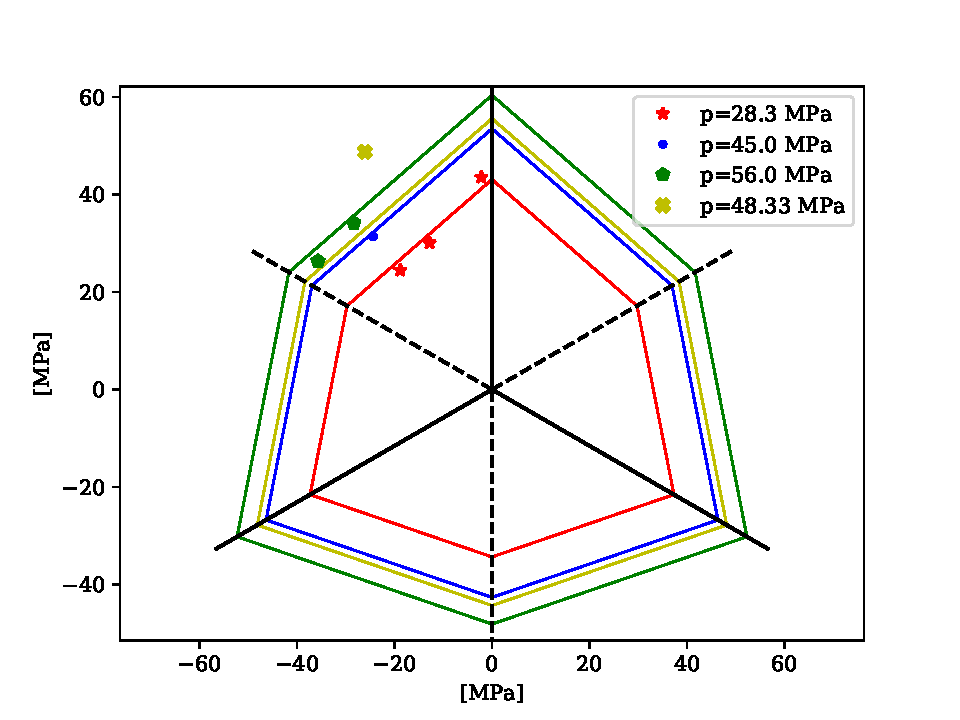
\includegraphics[width=0.5\columnwidth]{ch5/mc_pi_plane1}
    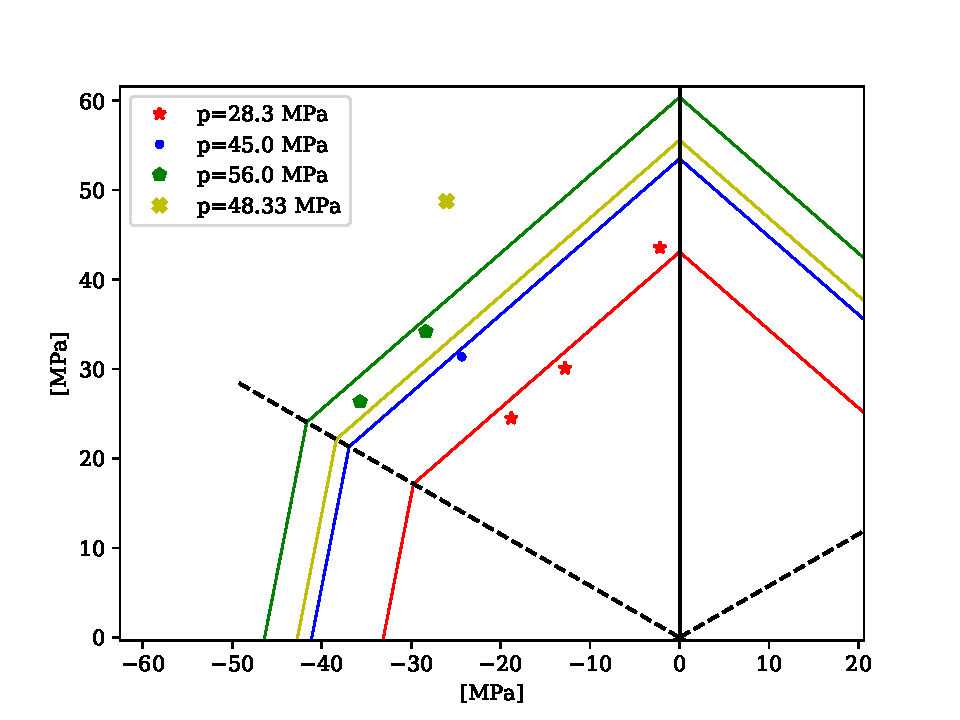
\includegraphics[width=0.9\columnwidth]{ch5/mc_pi_plane2}
    \caption{Mohr-Coulomb criterion failure surface in  $\pi$-plane}
    \label{fig5:mc_pi_plane}
\end{figure} 

The mean standard deviation misfit obtained for the Mohr-Coulomb failure criterion is $14.0$ [\si{\mega\pascal}]. 

%%%%%%%%%%%%%%%%%%%%%%%%%%%%%%%%%%%%%%%%%%%%%%%%%%%%%%%%%%%%%%
\subsection{Hoek-Brown failure criterion}

The Hoek-Brown failure criterion is also formulated in terms two principal stresses (cf. Equations \ref{eq2:HB-crit}) and unique strength parameters (i.e. $m$, $C_0$), therefore, the fitting was done using only axisymmetric triaxial compression tests results (i.e. $\theta = 0^\circ$). 

From this fitting, the strength parameter $m$ was determined and $V_0$ was computed: 

\begin{equation}
    m = 5.96 \quad \textrm{and} \quad C_0 = \SI{29.7}{\mega\pascal}
\end{equation}
\begin{equation}
    V_0 = \frac{C_0}{m} = \SI{4.98}{\mega\pascal}
\end{equation}

Knowing the strength parameters, the Hoek-Brown failure surface is plotted in the $(\sigma_3-\sigma_1)$ plane using Equations \ref{eq2:HBsig1_CTC} for the compression line and \ref{eq2:HBsig1_CTE} for extension (cf. Figure \ref{fig5:mc_sig1sig3}).

\begin{figure}[tb]
    \centering
    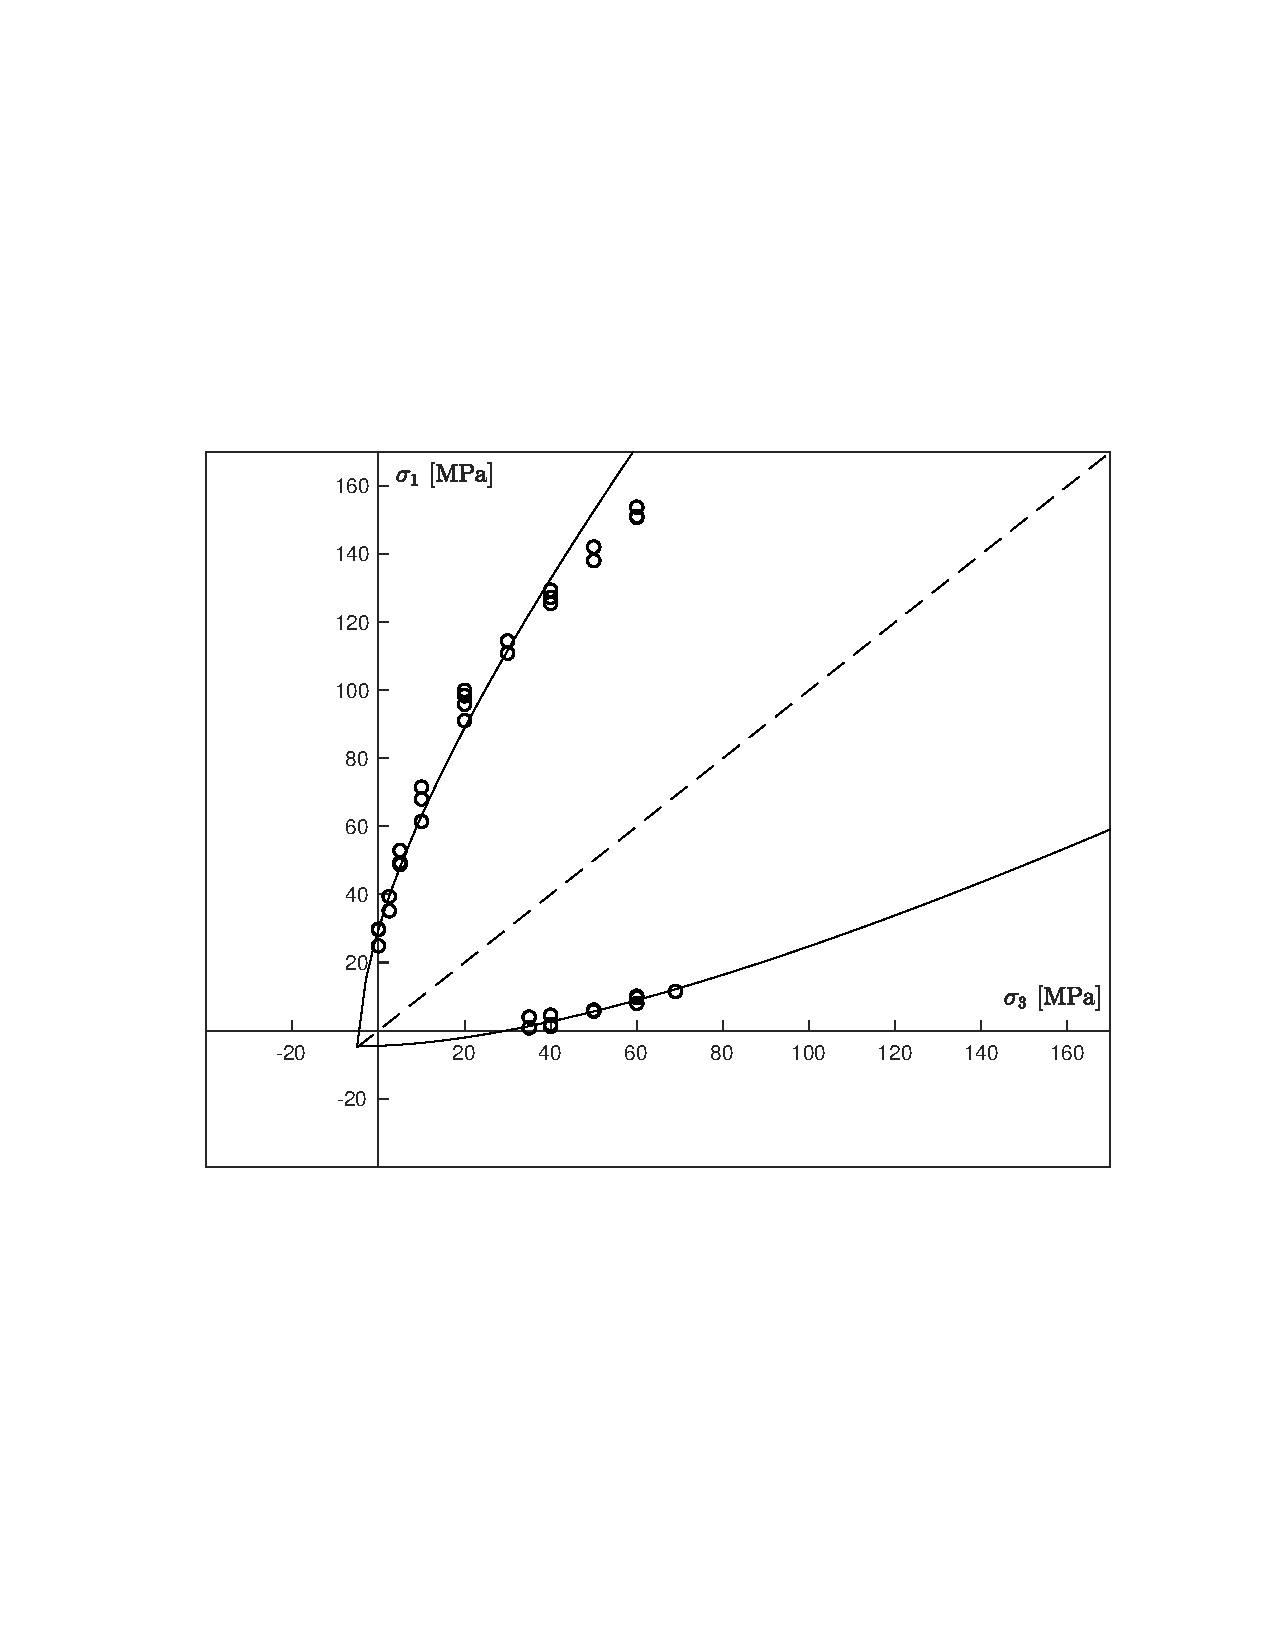
\includegraphics[width=0.8\columnwidth]{ch5/hb_sig1sig3}
    \caption{Hoek-Brown criterion failure surface in  $(\sigma_3-\sigma_1)$ plane}
    \label{fig5:hb_sig1sig3}
\end{figure} 

In the $(p-q)$ plane, the Hoek-Brown failure criterion is plotted using Equations \ref{eq2:HB-q-CTC} for compression and \ref{eq2:HB-q-CTE} for extension. These surfaces are expressed in terms of $m$ and $C_0$ previously defined. 

\begin{figure}[tb]
    \centering
    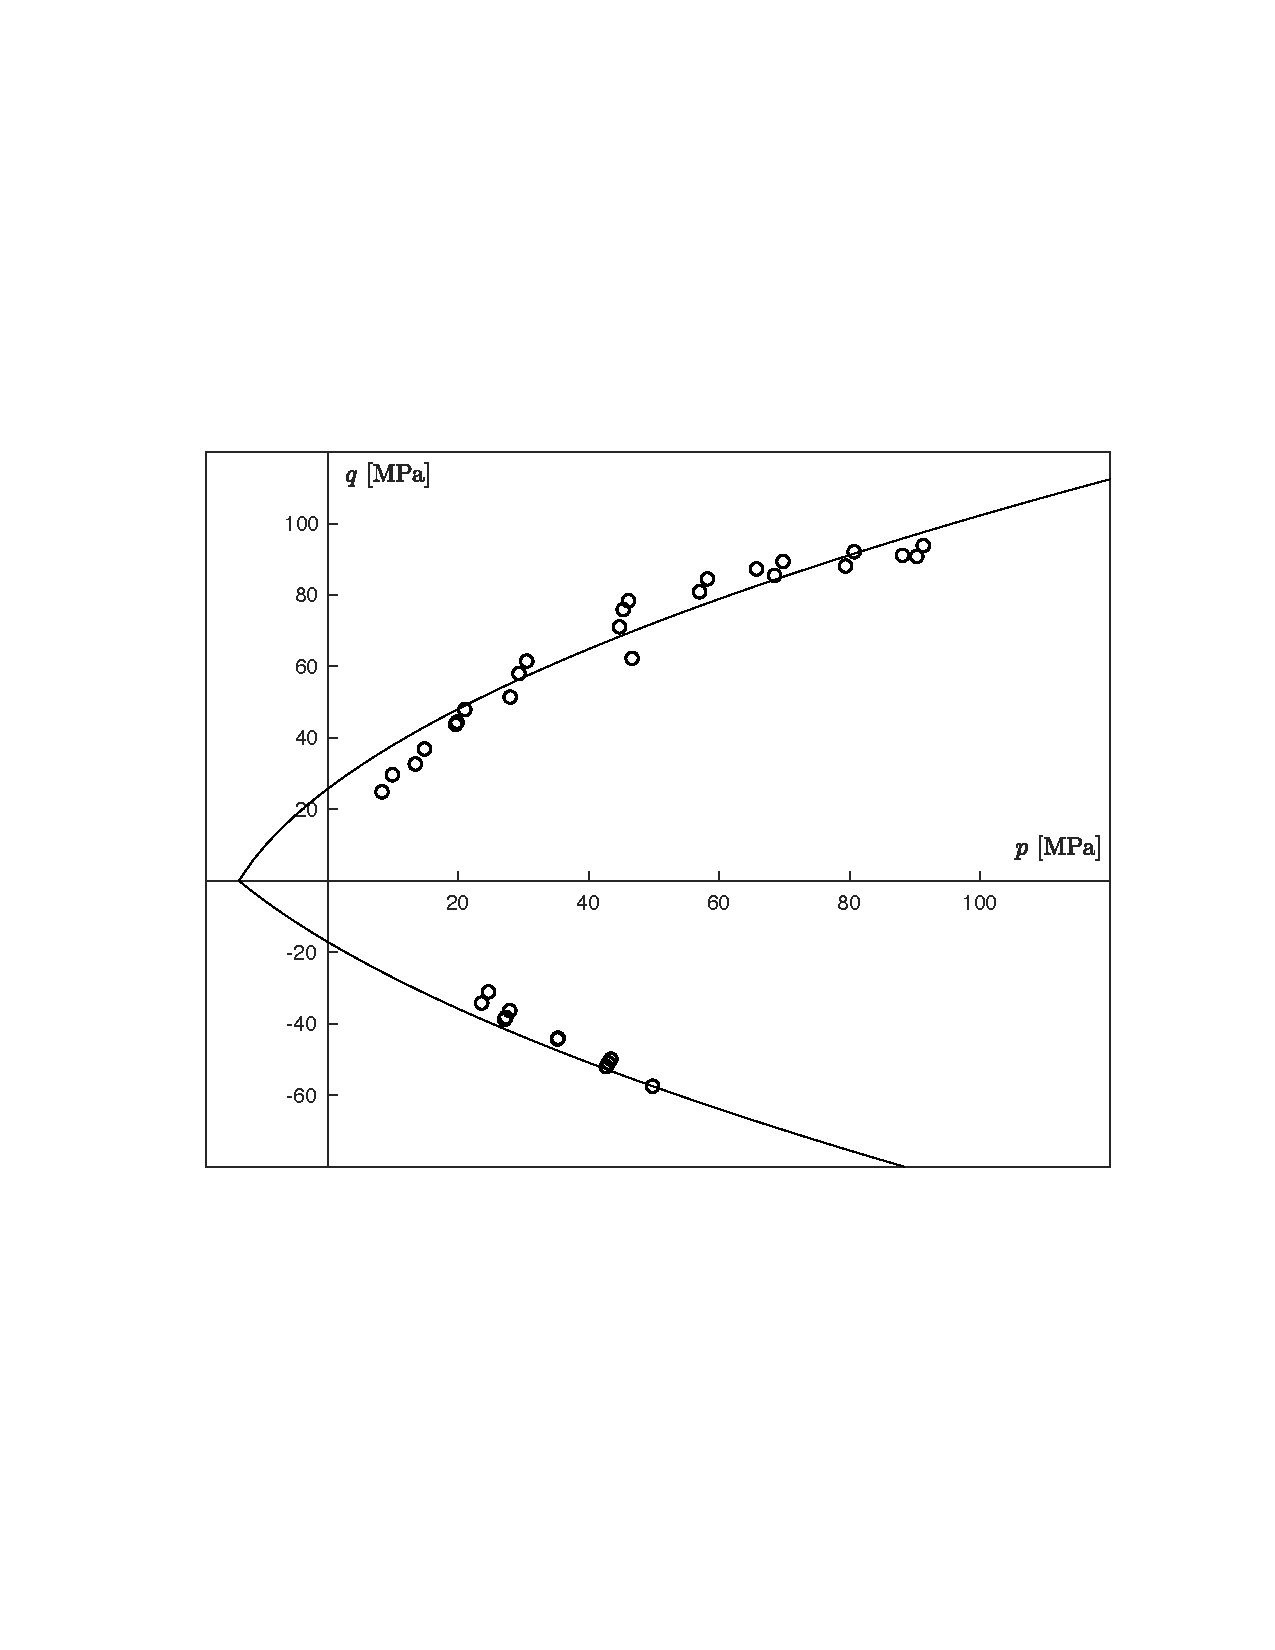
\includegraphics[width=0.8\columnwidth]{ch5/hb_pq}
    \caption{Hoek-Brown criterion failure surface in  $(p-q)$ plane}
    \label{fig5:hb_pq}
\end{figure} 

Finally, the Hoek-Brown criterion is presented in the $\pi$-plane, obtained following the procedure described in Section \ref{ch2:HB_pi}. Figure \ref{fig5:hb_pi_plane} shows Mohr-Coulomb failure criterion in the pi-plane at different values of the mean stress $p$.

\begin{figure}[tb]
    \centering
    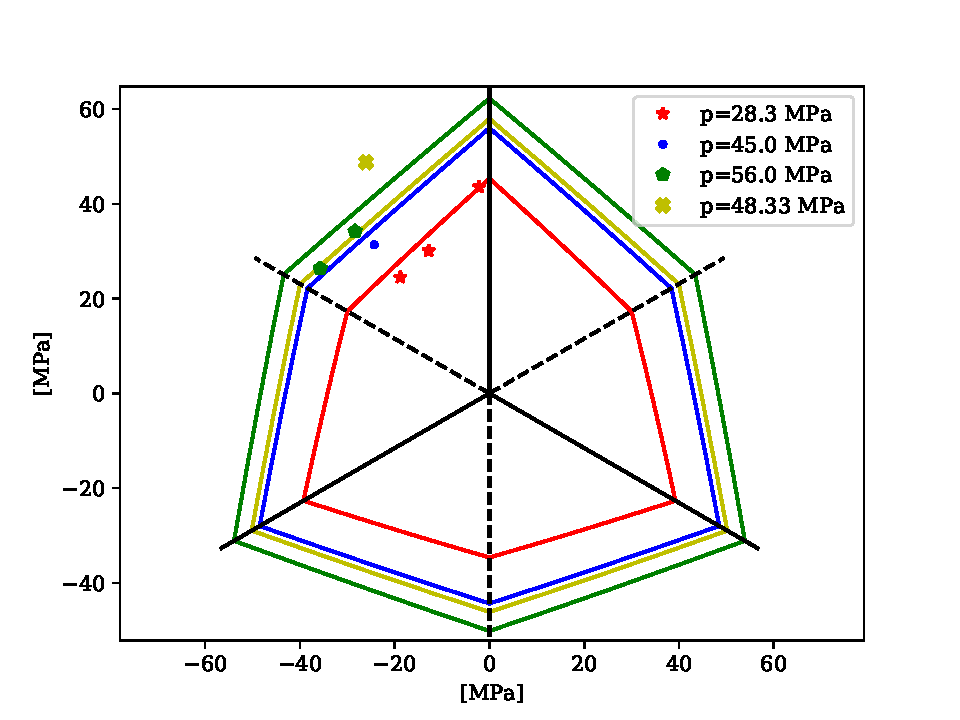
\includegraphics[width=0.5\columnwidth]{ch5/hb_pi_plane1}
    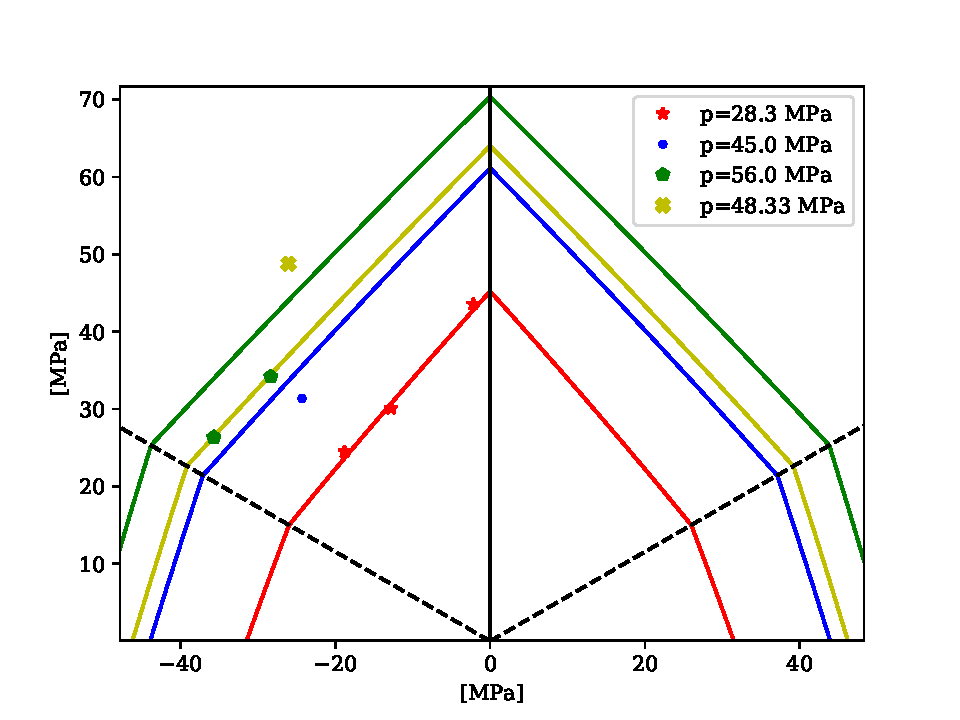
\includegraphics[width=0.9\columnwidth]{ch5/hb_pi_plane2}
    \caption{Hoek-Brown criterion failure surface in  $\pi$-plane}
    \label{fig5:hb_pi_plane}
\end{figure} 

The mean standard deviation misfit obtained for the Hoek-Brown failure criterion is $9.37$ [\si{\mega\pascal}]. 

%%%%%%%%%%%%%%%%%%%%%%%%%%%%%%%%%%%%%%%%%%%%%%%%%%%%%%%%%%%%%%
\subsection{Paul-Mohr-Coulomb failure criterion}

The fitting presented in this section is referred as the "3 parameters Paul-Mohr-Coulomb criterion", as it accounts only 
Contrary to the previous criteria, the Paul-Mohr-Coulomb failure criterion is formulated in terms the three principal stresses (cf. Equations \ref{eq2:PMC} and \ref{eq2:PMC_dev}) and non-unique strength parameters (i.e. $\phi_{c,e}$, $c_{c,e}$, $V_0$), therefore, the fitting was done using all tests results from the database (i.e. $\theta = 0^\circ$). 

From the least-square solution fitting describe in Chapter 2 (cf. Section \ref{ch2:pmcfit}, Equations \ref{eq2:PMCfinalform} and \ref{eq2:pmc_be}), the following solution could be obtained:
\begin{equation}
    x_1 = \frac{b_c}{V_0} = 0.81
\end{equation}
\begin{equation}
    x_2 = k = -0.91
\end{equation}
\begin{equation}
    x_3 = b_c = \SI{28.77}{\mega\pascal}
\end{equation}

Following Equations \ref{eq2:pmc_vo} to \ref{eq2:pmc_c}, the strength parameters for Paul-Mohr-Coulomb failure criteria could be computed:

\begin{equation}
    V_0 = \frac{0.81}{b_c} = \SI{35.62}{\mega\pascal}
\end{equation}
\begin{equation}
    b_e = \frac{2b_c}{(1-\sqrt{3}k)} = \SI{22.31}{\mega\pascal}
\end{equation}
\begin{equation}
    \phi_c = arcsin\left(\frac{3b_c}{6V_0+b_c}\right) = \SI{20.85}{\degree}
\end{equation}
\begin{equation}
    \phi_e = arcsin\left(\frac{3b_e}{6V_0-b_c}\right) = \SI{20.85}{\degree}
\end{equation}
\begin{equation}
    c_{c}=\frac{b_{c}\left(3-\sin \phi_{c}\right)}{6 \cos \phi_{c}} = \SI{13.57}{\mega\pascal}
\end{equation}
\begin{equation}
    c_{e}=\frac{b_{e}\left(3+\sin \phi_{e}\right)}{6 \cos \phi_{e}} = \SI{10.52}{\mega\pascal}
\end{equation}

Knowing the strength parameters, the Paul-Mohr-Coulomb failure surface could be plotted in the $(\sigma_3-\sigma_1)$ plane using Equations \ref{eq2:PMC_sig1sig3} to \ref{eq2:PMC_sig1sig3_Cce}. The graph obtained is presented in Figure \ref{fig5:pmc_sig1sig3}.

\begin{equation}
    M_c = \frac{1+\sin \phi_c}{1-\sin \phi_c} = 2.11
\end{equation}
\begin{equation}
    M_e = \frac{1+\sin \phi_e}{1-\sin \phi_e} = 2.08
\end{equation}
\begin{equation}
    C_c = \frac{2c_c\cos \phi_c}{1-\sin \phi_c} = \SI{39.38}{\mega\pascal}
\end{equation}
\begin{equation}
    C_e = \frac{2c_e\cos \phi_e}{1-\sin \phi_e} = \SI{30.31}{\mega\pascal}
\end{equation}

\begin{figure}[tb]
    \centering
    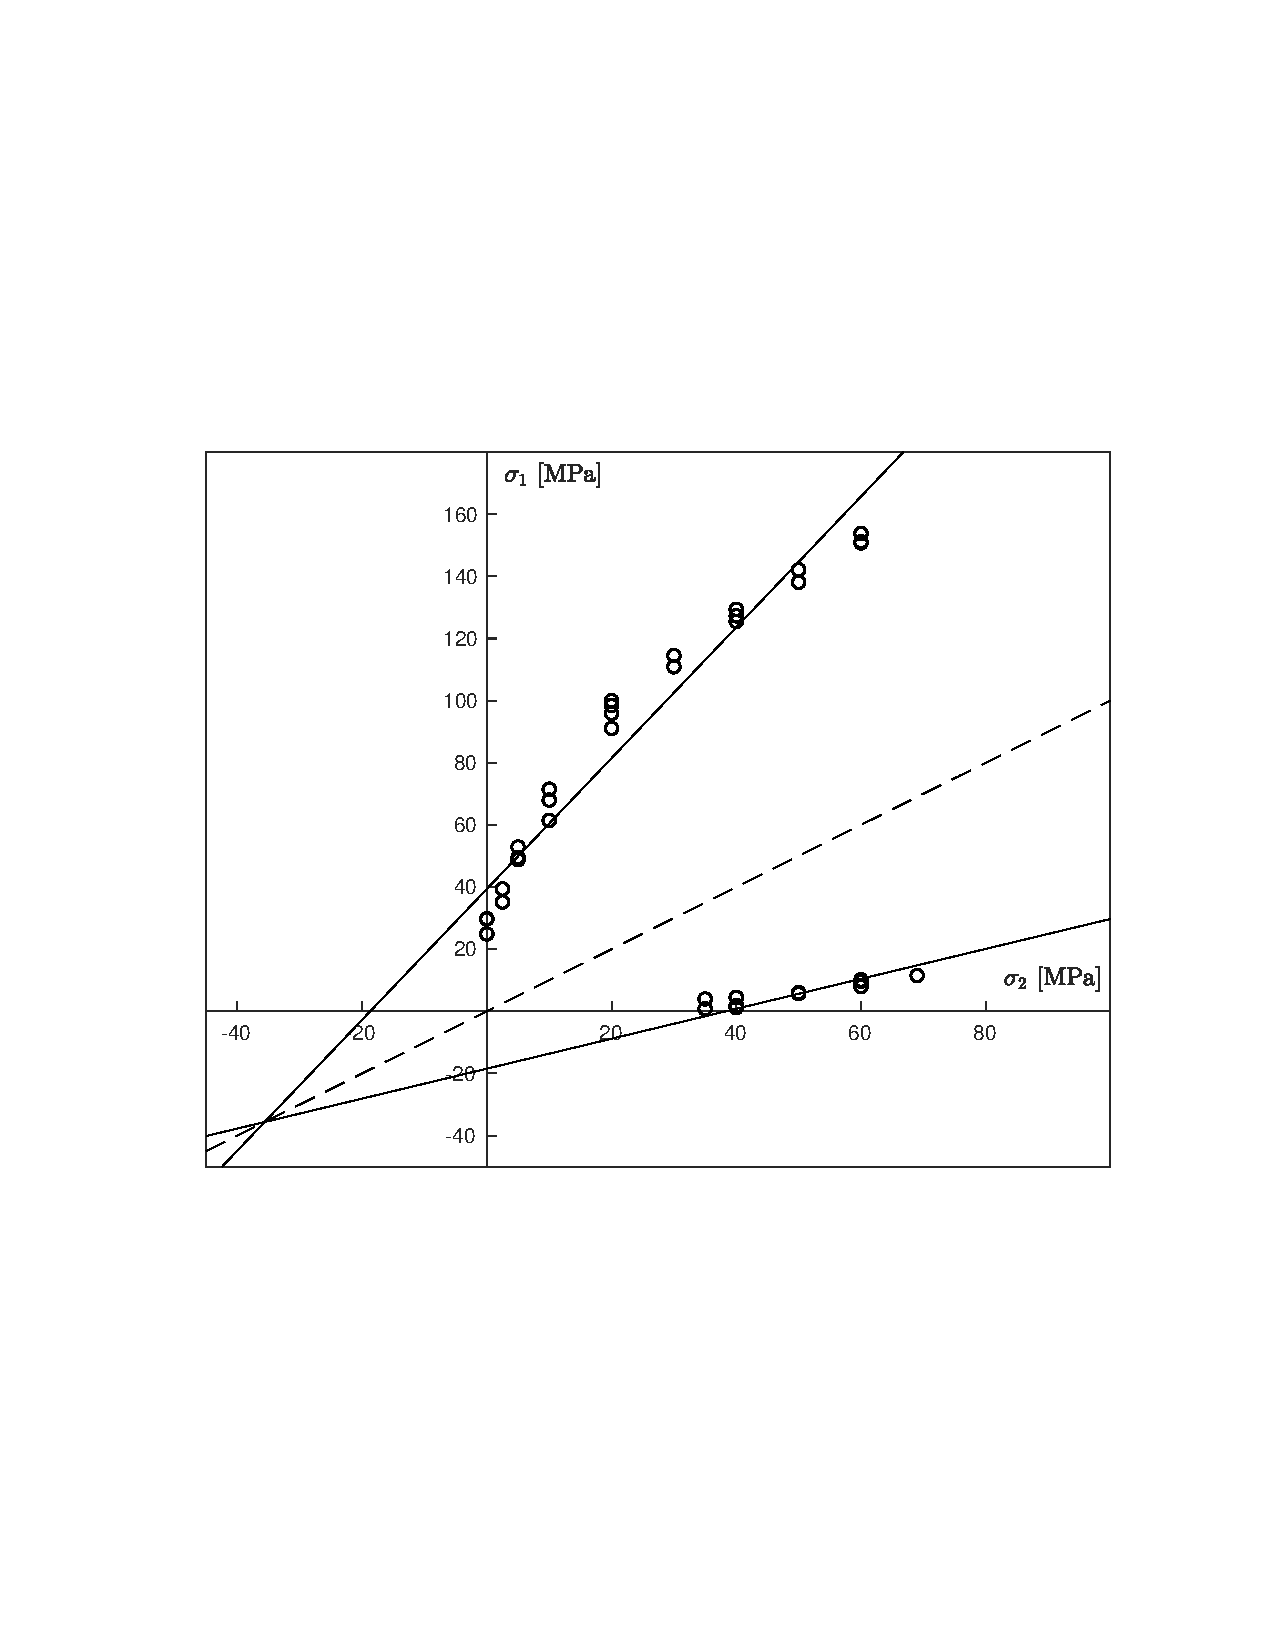
\includegraphics[width=0.8\columnwidth]{ch5/pmc3p_sig1sig3}
    \caption{Paul-Mohr-Coulomb criterion failure surface in  $(\sigma_3-\sigma_1)$ plane}
    \label{fig5:pmc_sig1sig3}
\end{figure}

The 

\section{Bi-linear Paul-Mohr-Coulomb failure criterion}\label{ch5:PMC}

Published data from rock testing in conventional triaxial and multi axial testing showed that the failure envelop is non-linear. This non-linearity can be approximated by fitting the experiments data using two planes instead of one, resulting in six parameters describing the envelop. 

The six-parameters fitting splits the data points in two sets in order to create two planes. These planes will give a better approximation of the failure envelop. The fitting procedure presented in 4.3.1. should then be applied to the two set of data points, resulting in different values of $\phi_c$,$\phi_e$ and $V_0$ for each plane.  

\section{Discussion}